\documentclass{beamer}
% \documentclass[handout,xcolor=pdftex,dvipsnames,table]{beamer}

\mode<presentation>
{
  \usetheme{Warsaw}
  \usecolortheme{whale}
  % or ...

  \setbeamercovered{transparent}
  % or whatever (possibly just delete it)
  \setbeamertemplate{navigation symbols}{}
}

\setbeamertemplate{itemize items}[ball]
\setbeamertemplate{itemize subitem}[triangle]
\setbeamertemplate{itemize subsubitem}[circle]
\setbeamercovered{transparent}

\usepackage{palatino} 
\usepackage{listings} % Gives syntax highlighting for python code. 
\usepackage{color} % Used for syntax highlighting. 
\usepackage{textcomp} % Used for syntax highlighting. 
\usepackage{caption}
\captionsetup{labelformat=empty,labelsep=none}
% This gives syntax highlighting in the python environment 
\definecolor{gray}{gray}{0.5} 
\definecolor{key}{rgb}{0,0.5,0} 
\lstset{
language=python,
basicstyle=\ttfamily\tiny, 
otherkeywords={1, 2, 3, 4, 5, 6, 7, 8 ,9 , 0, -, =, +, [, ], (, ), \{, \}, :, *, !}, 
keywordstyle=\color{blue}, 
stringstyle=\color{red},
showstringspaces=false,
alsoletter={1234567890},
otherkeywords={\ , \}, \{},
keywordstyle=\color{blue},
emph={access,and,break,class,continue,def,del,elif ,else,%
except,exec,finally,for,from,global,if,import,in,is,%
lambda,not,or,pass,print,raise,return,try,while},
emphstyle=\color{black}\bfseries,
emph={[2]True, False, None, self},
emphstyle=[2]\color{green},
emph={[3]from, import, as},
emphstyle=[3]\color{blue},
upquote=true,
morecomment=[s]{"""}{"""},
commentstyle=\color{gray}\slshape,
emph={[4]1, 2, 3, 4, 5, 6, 7, 8, 9, 0},
emphstyle=[4]\color{blue},
literate=*{:}{{\textcolor{blue}:}}{1}%
{=}{{\textcolor{blue}=}}{1}%
{-}{{\textcolor{blue}-}}{1}%
{+}{{\textcolor{blue}+}}{1}%
{*}{{\textcolor{blue}*}}{1}%
{!}{{\textcolor{blue}!}}{1}%
{(}{{\textcolor{blue}(}}{1}%
{)}{{\textcolor{blue})}}{1}%
{[}{{\textcolor{blue}[}}{1}%
{]}{{\textcolor{blue}]}}{1}%
{<}{{\textcolor{blue}<}}{1}%
{>}{{\textcolor{blue}>}}{1},%
numbers=none,
}

\newcommand{\putat}[3]{\begin{picture}(0,0)(0,0)\put(#1,#2){#3}\end{picture}}



\title[]{Python Workshop\\
Getting Started with Python}

\author[Fienen] % (optional, use only with lots of authors)
{M.N.~Fienen}
\institute[USGS] % (optional, but mostly needed)
{
  U.S. Geological Survey\\
  Wisconsin Water Science Center, Middleton, Wisconsin USA
  }

\date[UQ12] % (optional, should be abbreviation of conference name)
{USGS National Groundwater Workshop, August 2012}

\subject{Python}


\begin{document}

\begin{frame}
  \titlepage
\end{frame}

\begin{frame}{Outline}
\tableofcontents
\end{frame}

\section{Preliminaries}
\begin{frame}[fragile]
\frametitle{What is Python?}
\begin{itemize}
\item{Python is a high-level, general programming language (relying much on C underneath) that is interpreted at run time through a command-line interface or scripting.} 
\item {Python is free, open-source, and platform-independent.}
\item{Python has a massive user community worldwide and growing within USGS}
\end{itemize}
    \begin{figure}
    \putat{100}{-65}{
        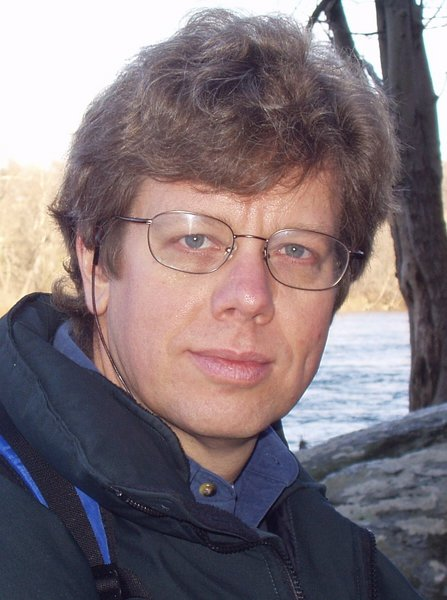
\includegraphics[width=2cm,height=2.68cm]{figures/Guido_van_Rossum.jpg}
	}
	\putat{80}{-75}{Guido van Rossum}
	
        
\includegraphics[width=3cm,height=.89cm]{figures/python.png}
        
    \end{figure}       
                  
\end{frame}

\begin{frame}[fragile]
\frametitle{Python Versions and Packages}
\begin{itemize}
\item{The two main version branches are 2.x and 3.x}
\item{We \emph{strongly} recommend sticking with 2.x \newline{}for now--Specifically \bf{2.7.3}}
\item{To do almost any substantial mathematics or statistics, you also need \texttt{numpy}}
\item{Basic 2-D graphics are possible using \texttt{matplotlib}}
\item{More advanced statistics are also available using \texttt{scipy}}
\item{Distributions already including many packages:}
\begin{itemize}
\item {pythonxy: for Windows only \url{http://pythonxy.com}
\includegraphics[scale=0.4]{figures/pythonxy.png}}
\item {EPD: Enthought Python Distribution for all Platforms \url{http://www.enthought.com}

\includegraphics[width=3cm,height=.86cm]{figures/enthought.png}}
\end{itemize}
\end{itemize}
\end{frame}

\section {Getting Help}
\begin{frame}[fragile]
\frametitle{Resources}
\end{frame}

\end{document}